% !TEX TS-program = xelatex
\documentclass[11pt,landscape,a4paper]{article}
\usepackage[normalem]{ulem}
\usepackage{amsmath}
\usepackage{graphicx}
\graphicspath{{./}}
\usepackage{tikz}
\usetikzlibrary{shapes,positioning,arrows,fit,calc,graphs,graphs.standard}
\usepackage[nosf]{kpfonts}
\usepackage[t1]{sourcesanspro}
\usepackage{multicol}
\usepackage{wrapfig}
\usepackage[top=0mm,bottom=1mm,left=0mm,right=1mm]{geometry}
\usepackage[framemethod=tikz]{mdframed}
\usepackage{microtype}
\usepackage{tabularx}
\usepackage{hhline}
\usepackage{makecell}
\usepackage{mathtools}
\usepackage{listings}

\DeclarePairedDelimiter{\ceil}{\lceil}{\rceil}

\newcommand\codeblue[1]{\textcolor{blue}{\code{#1}}}

\usepackage{lastpage}
\usepackage{datetime}
\yyyymmdddate
\renewcommand{\dateseparator}{-}
\let\bar\overline

\definecolor{myblue}{cmyk}{1,.72,0,.38}

\def\firstcircle{(0,0) circle (1.5cm)}
\def\secondcircle{(0:2cm) circle (1.5cm)}

\colorlet{circle edge}{myblue}
\colorlet{circle area}{myblue!5}

\tikzset{filled/.style={fill=circle area, draw=circle edge, thick},
outline/.style={draw=circle edge, thick}}

\pgfdeclarelayer{background}
\pgfsetlayers{background,main}

%\everymath\expandafter{\the\everymath \color{myblue}}
%\everydisplay\expandafter{\the\everydisplay \color{myblue}}


\renewcommand{\baselinestretch}{.8}
\pagestyle{empty}

\global\mdfdefinestyle{header}{%
  linecolor=gray,linewidth=1pt,%
  leftmargin=0mm,rightmargin=0mm,skipbelow=0mm,skipabove=0mm,
}

\newcommand{\header}{
  \begin{mdframed}[style=header]
    \footnotesize
    \sffamily
    CS4248 Finals Cheatsheet v1.0 (\today)\\
    by~Aadit Rahul Kamat,~page~\thepage~of~\pageref{LastPage}
  \end{mdframed}
}

\let\counterwithout\relax
\let\counterwithin\relax
\usepackage{chngcntr}

\usepackage{verbatim}

\usepackage{etoolbox}
\makeatletter
\preto{\@verbatim}{\topsep=0pt \partopsep=0pt }
\makeatother

\counterwithin*{equation}{section}
\counterwithin*{equation}{subsection}
\usepackage{enumitem}
\newlist{legal}{enumerate}{10}
\setlist[legal]{label*=\arabic*.,leftmargin=2.5mm}
\setlist[itemize]{leftmargin=3mm}
\setlist[enumerate]{leftmargin=3.5mm}
\setlist{nosep}
\usepackage{minted}

\def\code#1{\texttt{#1}}

\newenvironment{descitemize} % a mixture of description and itemize
{\begin{description}[leftmargin=*,before=\let\makelabel\descitemlabel]}
{\end{description}}

\newcommand{\descitemlabel}[1]{%
  \textbullet\ \textbf{#1}%
}
\makeatletter



\renewcommand{\section}{\@startsection{section}{1}{0mm}%
  {.2ex}%
  {.2ex}%x
{\color{myblue}\sffamily\small\bfseries}}
\renewcommand{\subsection}{\@startsection{subsection}{1}{0mm}%
  {.2ex}%
  {.2ex}%x
{\sffamily\bfseries}}
\renewcommand{\subsubsection}{\@startsection{subsubsection}{1}{0mm}%
  {.2ex}%
  {.2ex}%x
{\rmfamily\bfseries}}



\def\multi@column@out{%
  \ifnum\outputpenalty <-\@M
    \speci@ls \else
  \ifvoid\colbreak@box\else
    \mult@info\@ne{Re-adding forced
    break(s) for splitting}%
    \setbox\@cclv\vbox{%
      \unvbox\colbreak@box
    \penalty-\@Mv\unvbox\@cclv}%
  \fi
  \splittopskip\topskip
  \splitmaxdepth\maxdepth
  \dimen@\@colroom
  \divide\skip\footins\col@number
  \ifvoid\footins \else
    \leave@mult@footins
  \fi
  \let\ifshr@kingsaved\ifshr@king
    \ifvbox \@kludgeins
      \advance \dimen@ -\ht\@kludgeins
      \ifdim \wd\@kludgeins>\z@
        \shr@nkingtrue
      \fi
    \fi
    \process@cols\mult@gfirstbox{%
      %%%%% START CHANGE
      \ifnum\count@=\numexpr\mult@rightbox+2\relax
        \setbox\count@\vsplit\@cclv to \dimexpr \dimen@-1cm\relax
        \setbox\count@\vbox to \dimen@{\vbox to 1cm{\header}\unvbox\count@\vss}%
      \else
        \setbox\count@\vsplit\@cclv to \dimen@
      \fi
      %%%%% END CHANGE
      \set@keptmarks
      \setbox\count@
      \vbox to\dimen@
      {\unvbox\count@
        \remove@discardable@items
    \ifshr@nking\vfill\fi}%
    }%
    \setbox\mult@rightbox
    \vsplit\@cclv to\dimen@
    \set@keptmarks
    \setbox\mult@rightbox\vbox to\dimen@
    {\unvbox\mult@rightbox
      \remove@discardable@items
  \ifshr@nking\vfill\fi}%
    \let\ifshr@king\ifshr@kingsaved
  \ifvoid\@cclv \else
    \unvbox\@cclv
    \ifnum\outputpenalty=\@M
  \else
    \penalty\outputpenalty
  \fi
  \ifvoid\footins\else
    \PackageWarning{multicol}%
    {I moved some lines to
      the next page.\MessageBreak
      Footnotes on page
    \thepage\space might be wrong}%
  \fi
  \ifnum \c@tracingmulticols>\thr@@
\hrule\allowbreak \fi
  \fi
  \ifx\@empty\kept@firstmark
    \let\firstmark\kept@topmark
    \let\botmark\kept@topmark
  \else
    \let\firstmark\kept@firstmark
    \let\botmark\kept@botmark
  \fi
  \let\topmark\kept@topmark
  \mult@info\tw@
  {Use kept top mark:\MessageBreak
    \meaning\kept@topmark
    \MessageBreak
    Use kept first mark:\MessageBreak
    \meaning\kept@firstmark
    \MessageBreak
    Use kept bot mark:\MessageBreak
    \meaning\kept@botmark
    \MessageBreak
    Produce first mark:\MessageBreak
    \meaning\firstmark
    \MessageBreak
    Produce bot mark:\MessageBreak
    \meaning\botmark
  \@gobbletwo}%
  \setbox\@cclv\vbox{\unvbox\partial@page
  \page@sofar}%
  \@makecol\@outputpage
  \global\let\kept@topmark\botmark
  \global\let\kept@firstmark\@empty
  \global\let\kept@botmark\@empty
  \mult@info\tw@
  {(Re)Init top mark:\MessageBreak
    \meaning\kept@topmark
  \@gobbletwo}%
  \global\@colroom\@colht
  \global \@mparbottom \z@
  \process@deferreds
\@whilesw\if@fcolmade\fi{\@outputpage
    \global\@colroom\@colht
  \process@deferreds}%
  \mult@info\@ne
  {Colroom:\MessageBreak
    \the\@colht\space
    after float space removed
  = \the\@colroom \@gobble}%
  \set@mult@vsize \global
  \fi}
  \global\let\tikz@ensure@dollar@catcode=\relax

  \def\mathcolor#1#{\@mathcolor{#1}}
  \def\@mathcolor#1#2#3{%
    \protect\leavevmode
    \begingroup
    \color#1{#2}#3%
    \endgroup
  }

  \makeatother
  \setlength{\parindent}{0pt}

  \setminted{tabsize=2, breaklines}
  % Remove belowskip of minted
  \setlength\partopsep{-\topsep}


  \newcolumntype{a}{>{\hsize=1.5\hsize}X}
%   \newcolumntype{b}{>{\hsize=.25\hsize}X}

  \setlength\columnsep{1.5pt}
  \setlength\columnseprule{0.1pt}

\begin{document}
\setlength{\abovedisplayskip}{0pt}
\setlength{\belowdisplayskip}{0pt}


\tiny
\begin{multicols*}{4}
  \raggedcolumns
  
  \section{Regular Expressions and Finite State \ Automata}
  \subsection{Finite State Automaton}
  \begin{itemize}
  \item Formal definition: (Q, $\Sigma$, $q_0$, F, $\delta(q, i)$ ) where:
  \item 
    \begin{itemize}
        \item Q: set of states
        \item $\sigma:$ input alphabet
        \item $q_0:$ the start state
        \item F: the set of final state
        \item $\delta(q, i)$: transition function between the states
      \end{itemize}
  \end{itemize}
  \subsection{Deterministic Finite State Automaton}
  \begin{itemize}
    \item Accepts an input string if we run out of input and it is in an accepting state
    \item Exactly one transition for a given symbol from one state to another
  \end{itemize}
  \subsection{Non-Deterministic Finite State Automaton}
  \begin{itemize}
    \item Accepts an input string if there is at least some path to an accepting state that exhaust the input string
    \item Could have more than one transition for the same input symbol or transition to another empty state through an empty symbol
  \end{itemize}
  \subsection{Convert from NFSA to DFSA}
  \begin{itemize}
      \item Keep track of all states that can be transitioned from NFSA
      \item A state in converted DFSA denotes a combination of states in NFSA
  \end{itemize}
  
\section{Words, Spelling Errors and Edit Distance}
\subsection{Porter Stemming Algorithm}
\begin{itemize}
\item ATIONAL -> ATE
\item ING -> $\epsilon$
\item SSES -> SS
\end{itemize}
\subsection{Bayesian Classification}
\begin{align*}
c\hat = argmax_{c \in C} P(c|o)
       = argmax_{c \in C} \frac{P(o|c).P(c)}{P(o)}
       = argmax_{c \in C} P(o|c).P(c)
\end{align*}
where P(o|c) is the likelihood and P(c) is the prior
\subsection{Minimum Edit Distance}
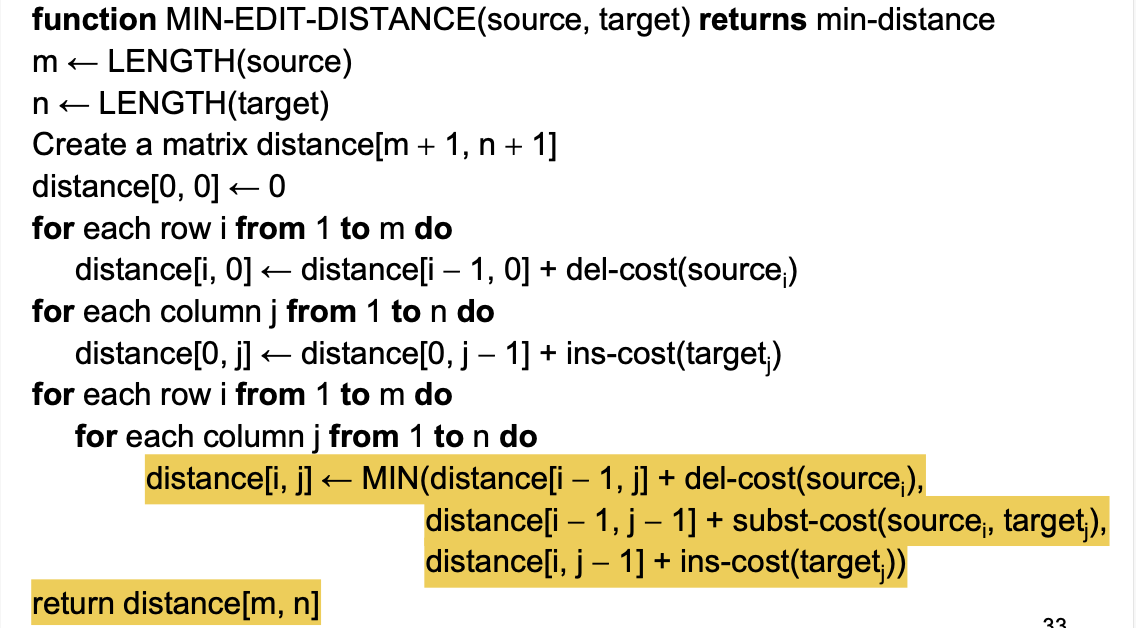
\includegraphics[width=0.8\columnwidth]{med}
\section{N-grams}
\subsection{N-gram approximation}
\begin{itemize}
\item $P(w_k | w_1,...,w_{k-1}) \approx P(w_k | w_{k - (n - 1)} , ..., w_{k - 2}, 2_{k - 1})$
\item MLE: $P(w_k | w_{k - (n - 1)},..., w_{k-2}, w_{k - 1}, w_k) = \\ \frac{C(w_{k - (n - 1)},..., w_{k-2}, w_{k - 1}, w_k)}{C(w_{k - (n - 1)},..., w_{k-2}, w_{k - 1})}$
\item bigram: n = 2 and trigram: n = 3
\end{itemize}
\subsection{Perplexity}
\begin{itemize}
\item $PP = m(w_1, .., w_n)^{-\frac{1}{n}} = \frac{1}{\sqrt[n]\{m(w_1, .., w_n)}$
\item For bigrams, $m(w_1, .., w_n) = \prod_{k=1}{n} P(w_k | w_{k - 1})$
\item Weighted average number of choices a random variable has to make (weighted average branching factor of a language)
\end{itemize}
\subsection{Smoothing}
\begin{itemize}
    \item Add k smoothing: $P(w|w_0) = \frac{C(w_0w) + k}{C(w_0) + kV}$
    \item Discount: $\frac{C*(w_0w)}{C(w_0w)}$
    \item Witten-Bell Smoothing:
    $P(w|w_0) =
    \begin{cases}
    \frac{C(w_0w)}{C(w_0) + T(w_0)}             & \text{if } C(w_0w) > 0 \\
    \frac{T(w_0)}{Z(w_0)(C(w_0) + T(w_0))}      & \text{if } C(w_0w) = 0
    \end{cases}$
    \item Kneser-Ney Smoothing for Bigram: 
    $\\P(w|w_0) =
    \begin{cases}
    \frac{C(w_0w) - D}{C(w_0)}       & \text{if } C(w_0w) > 0\\
    \frac{\alpha(w). |\{w': C(w'w_0) > 0\}}{\sum_{w}{|\{w': C(w' w) > 0\}|}}  & \text{if } C(w_0w) = 0
    \end{cases}$
\end{itemize}
\subsection{Entropy}
\begin{itemize}
\item $H(x) = - \sum_{x \in X}{p(x) log_2p(x)}$
\item Entropy for a language: $H(L) = lim_{n -> \inf}\frac{-1}{n}{log_2p(w_1, ..., w_n)}$
\item Cross Entropy: $H(p, m) = lim_{n -> \inf}\frac{-1}{n}\sum_{w \in L}{p(w_1,..., w_n) log_2 m(w_1, .., w_n)} $
\item Relation between Perplexity and Entropy: $\\Perplexity = 2^{H} = 2^{\frac{-1}{n} log_2 m(w_1, .., w_n)} = m(w_1, .., w_n)^{\frac{1}{n}}$
\end{itemize}


\section{POS Tagging}

\subsection{Stochastic POS Tagging}
\begin{itemize}
\item $T\hat = argmax_{t_1, .., t_T}{\prod_{i = 1}{T} P(t_i | t_{i - 1}). P(w_i | t_i). P(</s> | t_T)}$
\item Time Complexity: $O(T.N^T)$
\end{itemize}

\subsection{Viterbi (Dynamic Programming)} 
\begin{itemize}
\item $v_t(j) = max_{i=1}{N}a_{ij}b_{j}(o(t))$
where $a_{ij}$ is the transition probability, $b_{j}$ is the observation likelihood of observation $o(t)$
\item Time Complexity: $O(N^2)$
\end{itemize}

\subsection{Penn Treebank POS Tags}
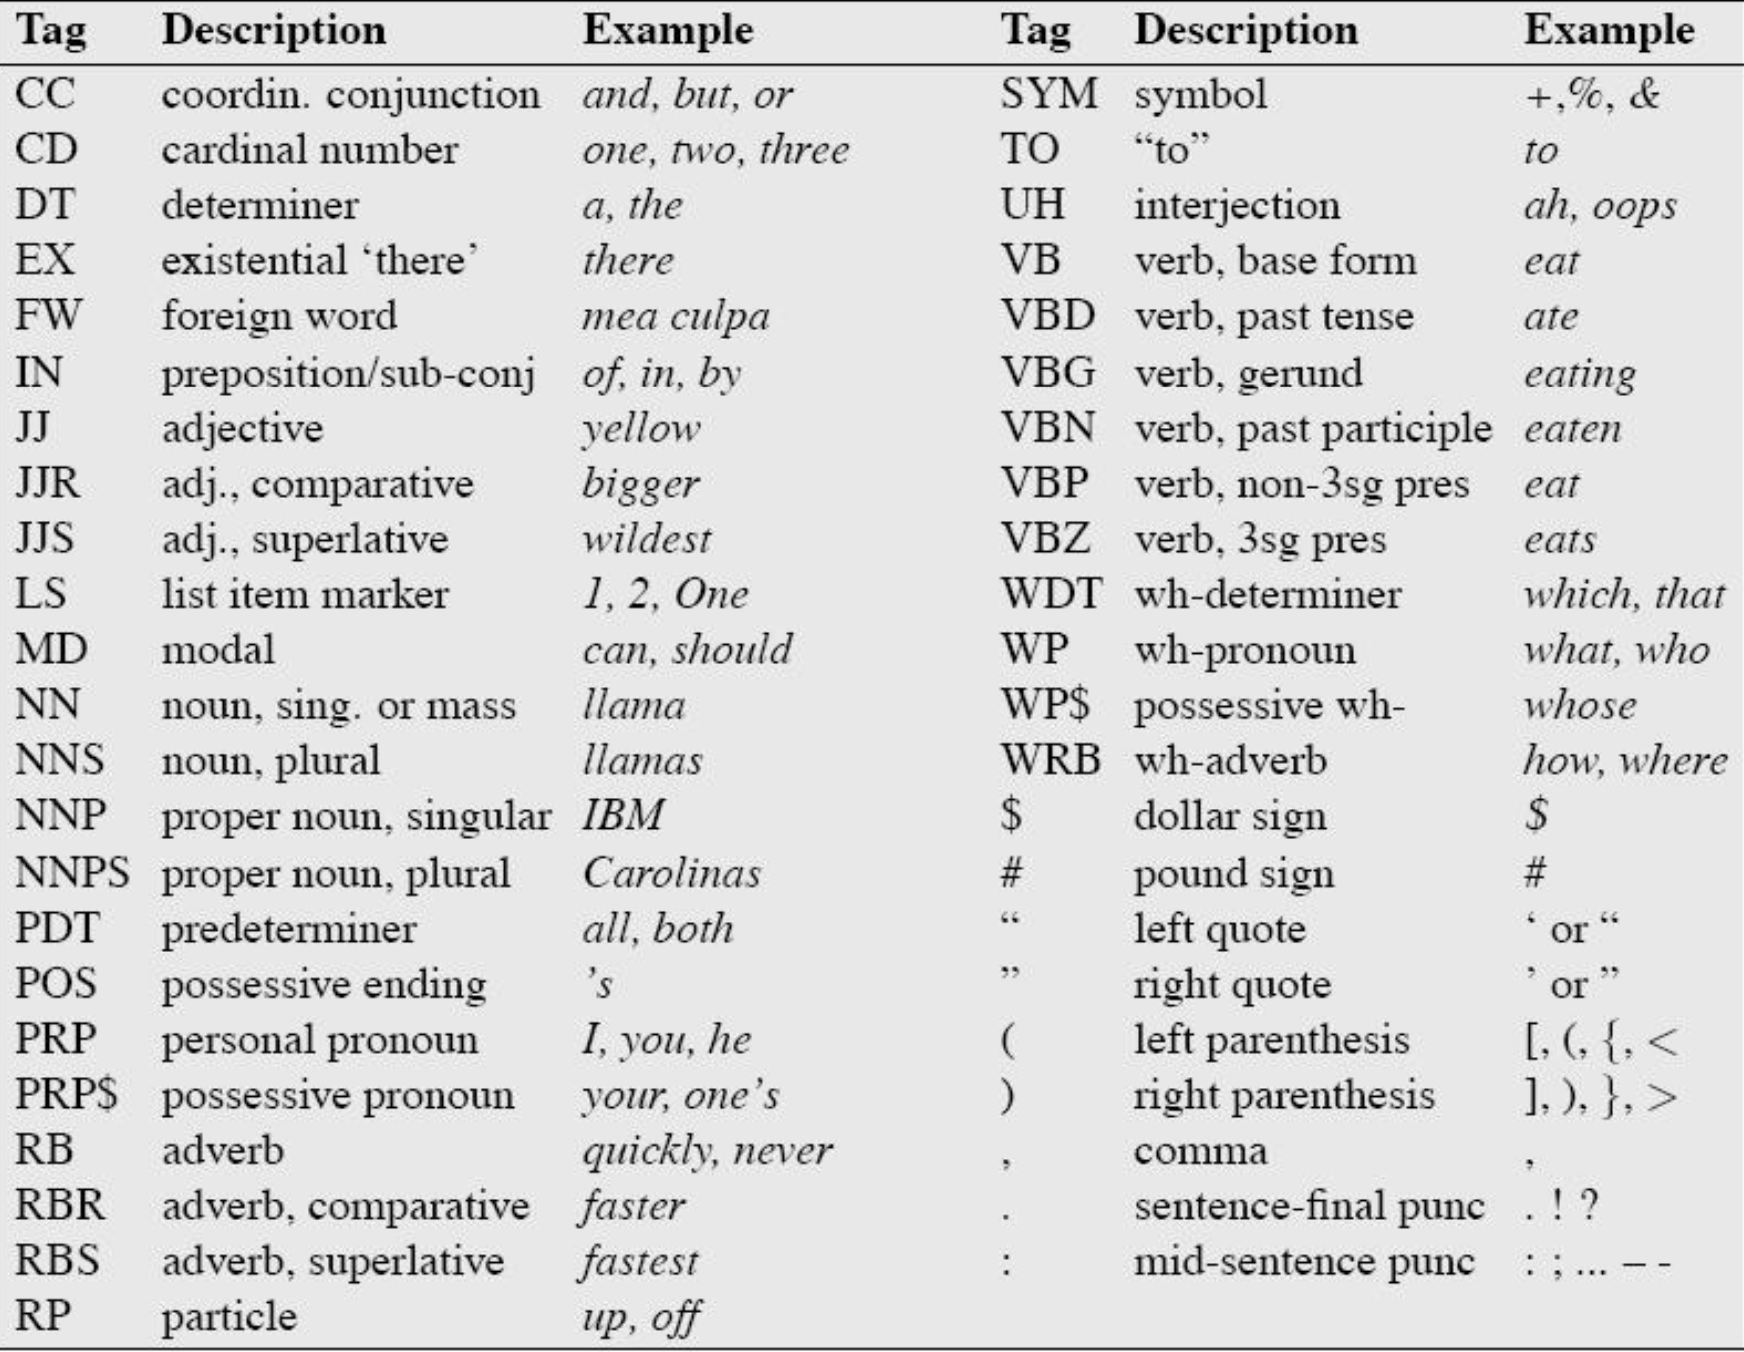
\includegraphics[width=0.8\columnwidth]{penn-treebank}


\section{Neural Networks}
\subsection {Multi Layer Perceptron}
\begin{align*}
NN_{MLP2}(x) = (g^2(g^1(xW^1 + b^1)W^2 + b^2))W^3 + b^3 \\
h^1 = g^1(xW^1 + b^1) \\
h^2 = g^2(xW^2 + b^2) \\
y = h^2W^3 + b^3
\end{align*}
\subsection {Activation Functions}
\begin{itemize}
    \item RELU(x) = $g(x) = max(0, x)$
    \item Sigmoid: 
    $\sigma(x) = \frac{1}{1 + e^{-x}}$, $\sigma'(x) = \sigma(x) (1 - \sigma(x))$
    \item Tanh:
    $tanh(x) = \frac{e^x + e^{-x}}{e^x - e^{-x}}$, $tanh'(x) = 1 - (tanh(x))^2$
    \item HardTanh: 
    $hardtanh(x) = 
    \begin{cases}
     -1      & x < -1 \\
      1 & x > 1  \\
      x  & \text{otherwise} \\
    \end{cases}$
\end{itemize}
\subsection {Loss Functions}
\begin{itemize}
    \item Cross Entropy Loss:
    $L_{logistic}(\hat{y}, y) = -y log_2(\hat{y}) - (1-y) log_2(1-\hat{y})$ 
    where $y \in \{0,1\}$ for binary classification
    \item For multi class classification (C > 2), 
    $L_{logistic}(\hat{y}, y) = \sum_{-i}^{C}{t_ilog_2(\hat{y}_{t})}$
    \item Softmax Loss: 
    $L_{softmax}(\hat{y}, y) = \frac{e^{\hat{y}_[i]}}{\sum_j{e^{\hat{y}_[j]}}}$, squishes range of values to (0, 1), a probability distribution
    \item Squared (quadratic) Loss: 
    $L_{squared}(\hat{y}, y) = 0.5 *(\hat{y} - y)^2$
    \item Hinge Loss:
    $L_hinge(\hat{y}, y) = max(0, 1 - \hat{y} * y)$
\end{itemize}
\subsection {Gradient Descent}
\begin{align*}
w_i = w_i - \alpha \frac{\delta L}{w_i}
\frac{\delta L}{w_m} = \sum_{i=1}{N}\frac{\delta L}{\delta x_i} \frac{\delta x_i}{\delta w_m}
\end{align*}

\section{Word Embeddings}

\subsection{Word2Vec}
\begin{align*}
    s(w, c) = w . c \\
    P(+ | t, c) = \frac{1}{1 + e^{-t.c}} \\
    P(- | t, c) = 1 - P(+ | t, c) = \frac{e^{-t.c}}{1 + e^{-t.c}}
\end{align*}
\subsection{Choosing noise words}
\begin{itemize}
\item $P_{\alpha}(w) = \frac{count(w)^{\alpha}}{\sum_w'{count(w')^{\alpha}}}$
where count is the unigram frequency. In practice, \$alpha\$ value of 0.75
works quite well.
\item Maximize objective function: 
$\\ \sum_{(w, c) \in D} {log_2 P(+ | t, c) + \sum_{(w, c) \in D} log_2 P(- | t, c)}$
\end{itemize}

\subsection{CBOW}
\begin{itemize}
\item $c= \sum_i{c_i}$
\item $log P(+ | w,c_{1:k}) = log \frac{1}{1 + e^(\sum_{i=1..k} w.c_i)}$
\end{itemize}

\subsection{Skip-gram}
\begin{itemize}
\item $P(+ | w,c_{1..k}) = \prod_{i=1}^{k}{\frac{1}{1 + e^{-w.c_i}}}$
\item $P(+ | w,c_{1..k}) = \sum_{i=1}^{k} {log \frac{1}{1 + e^{-w.c_i}}}$
\end{itemize}

\subsection{Cosine similarity}
\begin{itemize}
\item $sim_{cos}(u, v) = \frac{\textbf{u}.\textbf{v}}{\|\|\textbf{u}\|\|_{2}\|\|\textbf{v}\|\|_{2}}$
\item $analogy(m: w -> k : ?) = argmax_{v \in V \\ \{m, w, k\}}{cos(v, k - m + w)}$
\end{itemize}
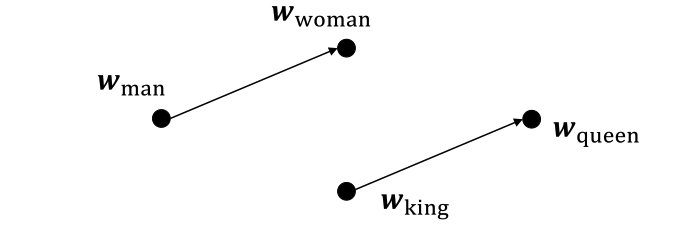
\includegraphics[width=0.8\columnwidth]{word-vector-algebra}

\section {CNN}
\subsection{Why is it used?}
\begin{itemize}
\item Identify informative ngrams
\item Consider local ordering patterns
\end{itemize}
\subsection{Process}
\begin{itemize}
    \item Apply non linear learned function (filter) over each k-word sliding window
    \item Apply l filters to get l-dimensional vector
    \item Combine vectors from different windows using pooling
    into single l-dimensional vector
    \item Feed single l-dimensional vector into neural network for prediction
\end{itemize}
\subsection{Convolution}
\begin{itemize}
    \item Narrow convolution (no padding): m = n - (k - 1)
    \item Wide convolution (padding k - 1 to each side) : m = n + (k - 1)
\end{itemize}
\subsection{Pooling}
\begin{itemize}
    \item Max pooling: 
    $c_j = max_{1 <= i <= m} p_{i_{[j]}}  \forall j \in [1, l]$
    \item Average pooling: 
    $\frac{1}{m}{\sum_{i = 1}^{m}{p_{i}}}$
\end{itemize}

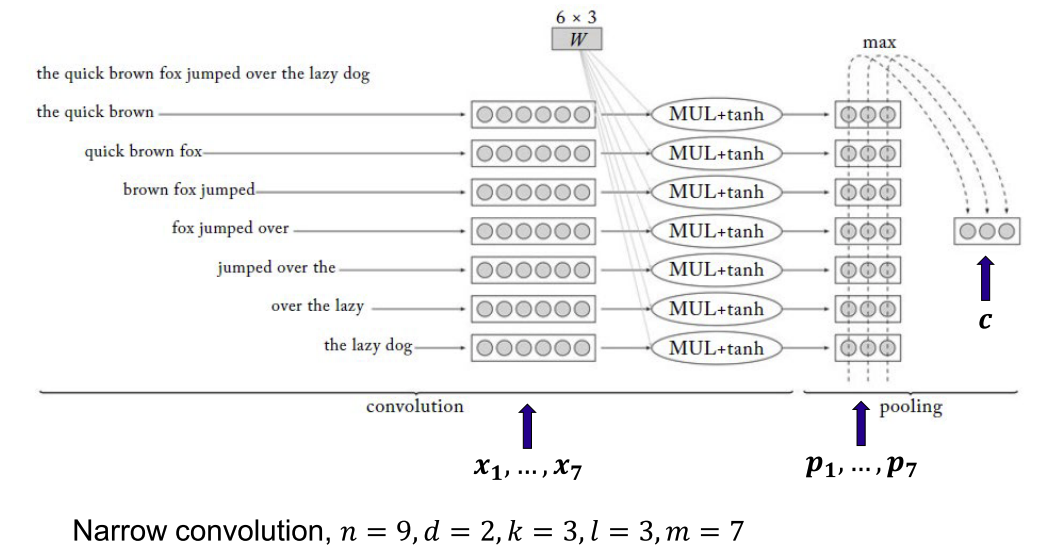
\includegraphics[width=0.8\columnwidth]{convolution}

\section {RNN}
\subsection{Why is it used?}
\begin{itemize}
\item Capture subtle patterns and regularities in sequences
\item Model non-Markovian dependencies
\end{itemize}
\subsection{RNN Abstraction}
\begin{align*}
 RNN^*(x_{1:n}:s_0) = y_{1..n} \\
 s_i = R(s_{i - 1}, x_i) \\
 y_i = o(s_i)
\end{align*}
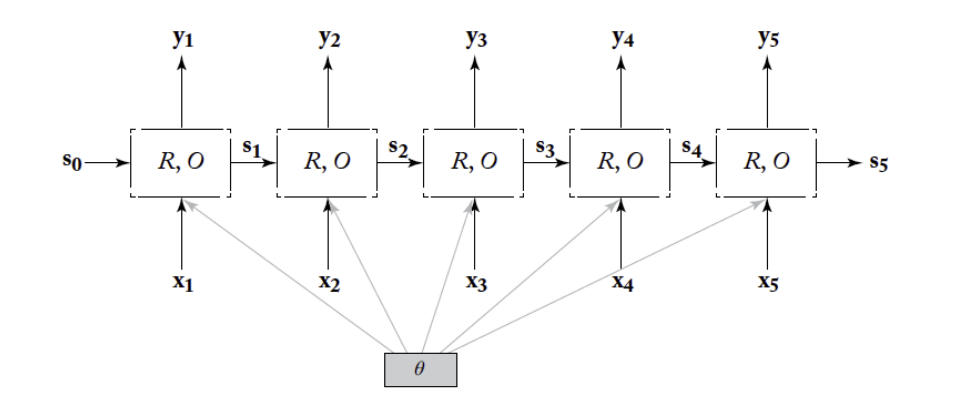
\includegraphics[width=0.8\columnwidth]{rnn-unrolled}
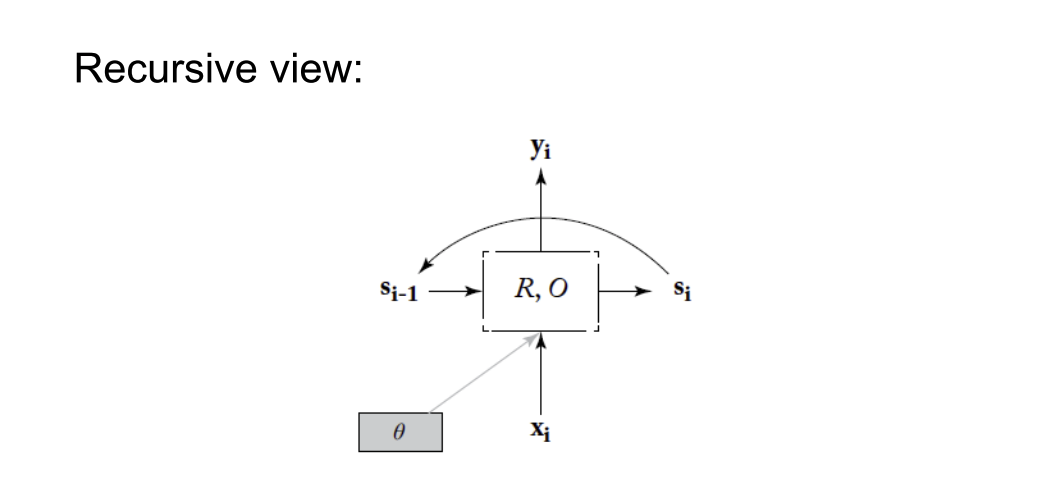
\includegraphics[width=0.8\columnwidth]{rnn-recursive}

\subsection{Elman RNN}
Sensitive to the order of the words
\begin{align*}
y_i  = O_RNN(s_i) \\
x_i \in R^{d_x}, S_i \in R^{d_s}, W\in R^{(d_x + d_s).d_s}, b \in R^d_s
\end{align*}

\subsection{CBOW RNN}
Does not take into account order of words
\begin{align*}
    s_i = R_{CBOW}(s_{i - 1}, x_i) = s_{i - 1} + x_i \\
    y_i = O_{CBOW}(s_i)
\end{align*}

\section{Seq2Seq}
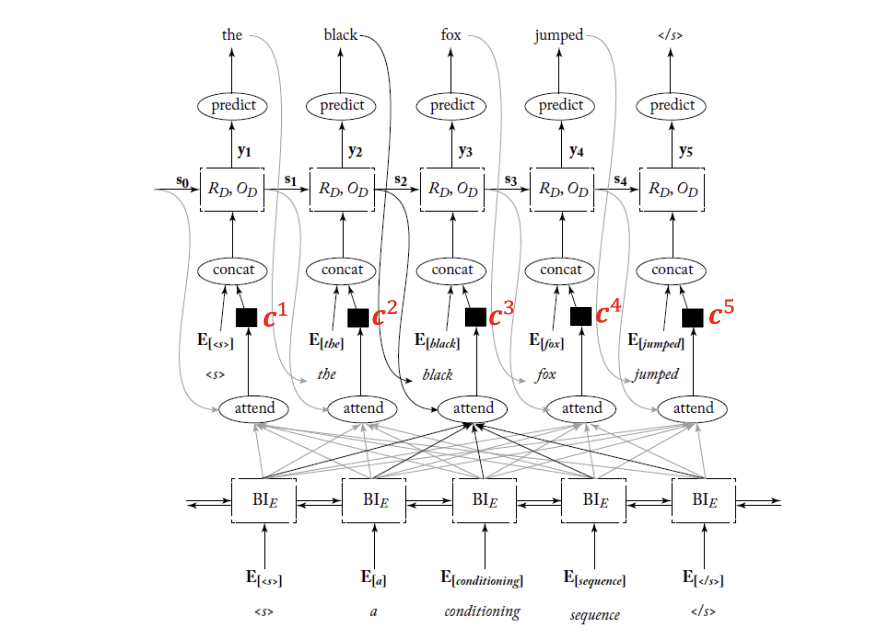
\includegraphics[width=0.8\columnwidth]{seq2seq}
\begin{align*}
    s_i = R_{dec}(s_{j - 1}, [\hat{t_j}; c^j]) \\
    y_j = O_{dev}(s_j) \\
    P(t_{j + 1}\hat | \hat{t_{1:j}},  x_{1:n}) = softmax(MLP^{out}(y_j)) \\
    c_{1:n} = biRNN_{enc}^{*}(x_{1:n}) \\
    \alpha^{j}_{[i]} = v.tanh([s_{j - 1};c_i] U + b) \\
    \alpha^{j}_{[i]} = softmax(\alpha^{j}_{[1]}, ..., \alpha^{j}_{[n]}) \\
    c^{j} = \sigma_{i=1}^{n}{\alpha_[i]^{j} . c_i} \text{(attend)} \\
\end{align*}

\section{Grammars}
\subsection{CFG}
$G = (N, \Sigma, P, S)$
\begin{itemize}
    \item N - terminal symbols
    \item $\Sigma$ - non-terminal symbols
    \item P - a -> A where $a \in N, A \in (\Sigma \cup  N)^* $
\end{itemize}
\subsection{CNF}
\begin{itemize}
    \item A -> BC or A -> a
    \item No $\epsilon$
\end{itemize}
\subsection{Equivalence}
\begin{itemize}
    \item Strong equivalence: $L(G1) = L(G2)$ and same phrase structure
    \item Weak equivalence: $L(G1) = L(G2)$ but different phrase structures
\end{itemize}
\subsection{Convert to CNF}
\begin{itemize}
    \item Copy all conforming rules to the new grammar unchanged
    \item Convert terminals within rules to dummy non-terminals
    \item Convert unit-productions 
    \item Binarize all rules and add to new grammar
\end{itemize}
\subsection{Converting Phrase Structure to Untyped Dependency}
\begin{itemize}
    \item Find the head (head child is underlined) and pass it up the tree
\end{itemize}
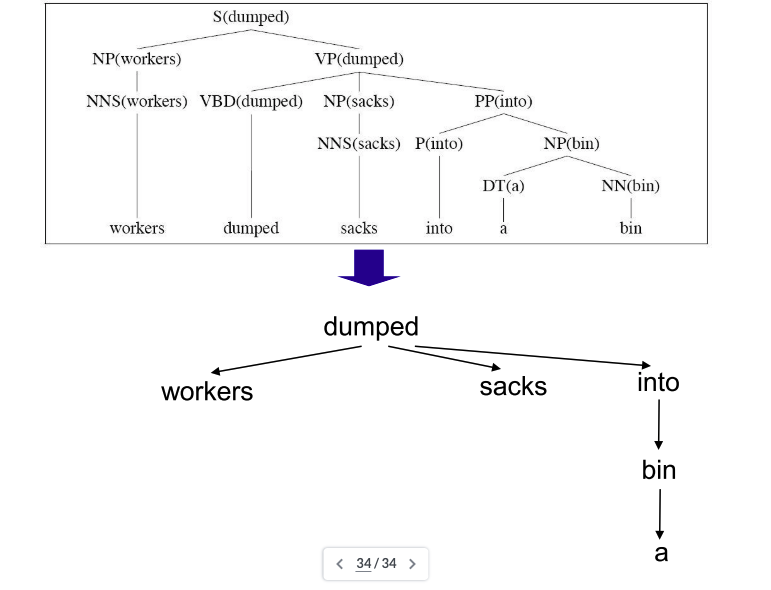
\includegraphics[width=0.8\columnwidth]{phrase-structure-to-untyped-dependency}

\subsection{Parsing}
\begin{itemize}
    \item Top down parsing: Goal directed, begin from start symbol and then derive parse tree for the given sentence consisting of terminals 
    \item Bottom up parsing: Data directed, start form   the terminals in a sentence and derive parse tree by tracing  up to the start symbol.
\end{itemize}

\subsection{Ambiguity}
\begin{itemize}
    \item Attachment Ambiguity: Ambiguity on how a verb phrase is split up based on the rules in the CFG (VP -> V NP PP or VP ->  V PP for example)
    \item Coordination Ambiguity: Ambiguity depending on how the Noun Phrase is split
    \item Noun Phrase Bracketing Ambiguity: Ambiguity depends on how the Noun Phrase is split 
\end{itemize}

\subsection{Parsing Algorithms}
\subsubsection{CKY algorithm}
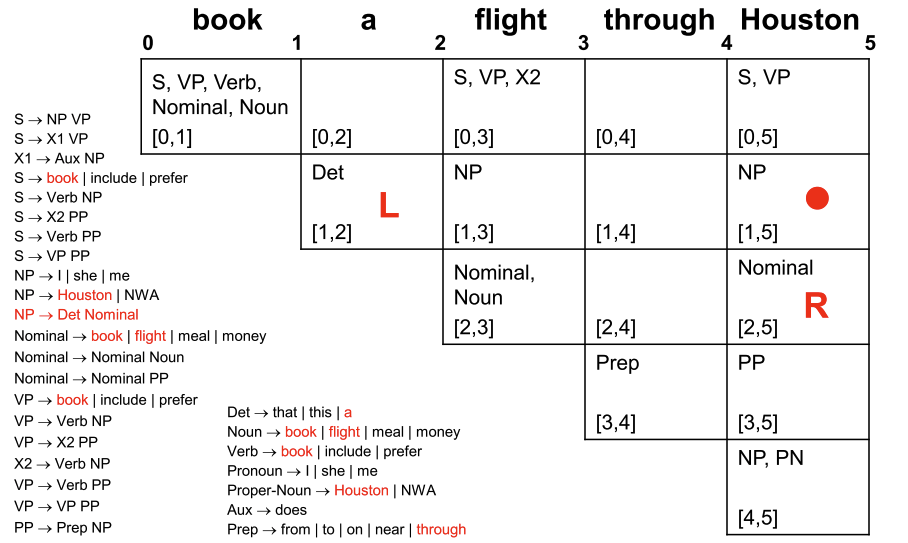
\includegraphics[width=0.8\columnwidth]{cky}
\begin{itemize}
    \item Bottom-up dynamic programming
    \item Grammar must be in CNF
    \item Time Complexity: $O(n^3)$, Space Complexity: $O(n^2)$
    \item Probabilistic version: most probable parse stored based on taking the maximum of probabilities calculated
    using the assigned probabilities for each production in the Grammar for regular CKY
\end{itemize}
\subsubsection{Earley Algorithm}
\begin{itemize}
    \item Top-down dynamic programming
    \item Grammar need not be in CNF
    \item Scan sentence from left to right
    \item Predictor: Create new states from original states using grammar
    (e.g. Given S -> .VP [0, 0], add VP -> .Verb [0, 0] and VP ->.Verb NP [0, 0])
    \item Scanner: Use predicted POS to incorporate the next word
    (e.g. Given the state VP -> .Verb NP [0, 0], add Verb -> book. [0, 1])
    \item Completer: Find and advanced previously created states looking for non-terminal at this position
    (e.g. Given stated NP -> Det Nominal.[1, 3] and VP -> Verb.NP [0, 1] and 
    add the new state VP -> Verb NP. [0, 3])
    \item Time Complexity: $O(n^3)$ maximum but tends to perform better, Space Complexity: $O(n)$
\end{itemize}

\section{Statistical Parsing}
\subsection{PCFG}
\begin{itemize}
    \item $P(T, S) = \prod_{t \in T}$ p (r(n)) where r(n) represents the rules of CFG applicable to the parse trees
    \item $T\hat(S) = argmax P(T)$
\end{itemize}

\subsection{Parse Tree Scoring}
\begin{itemize}
    \item $s_tree(T) = \sigma_{(i, j, l) \in T}{s(i, j, l)}$
    \item Feed sentence through bidirectional LSTM and then a Dense NN and score
    based on loss
    \item Dynamic Programming:
    \begin{align*}
        s_{best}(i, j) = max_l [s(i, j, l)] if j - i = 1 \\
        s_{best}(i, j) = max_l [s(i, j, 1)] + max_k[s_{best}(i, k) + s_{best}(k, j)]
    \end{align*}
    \item Best scored tree: $\hat{T} = argmax_{T}[s_{tree}(T)]$
\end{itemize}

\section{Semantics}
\subsection{First Order Logic}
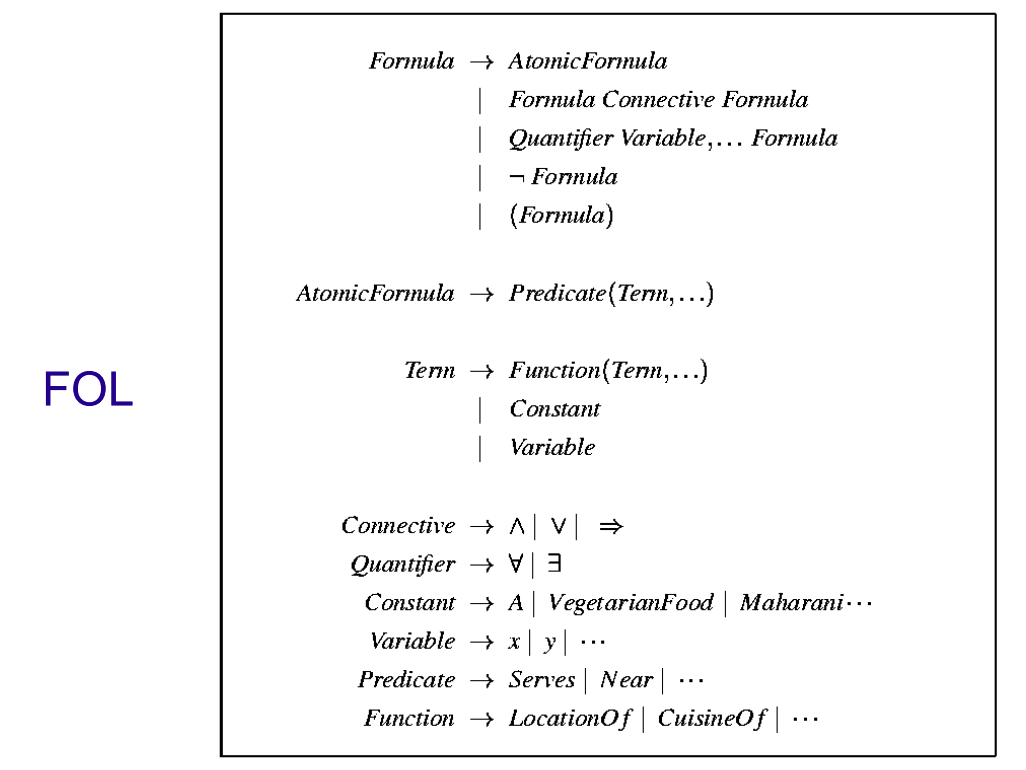
\includegraphics[width=0.8\columnwidth]{fol}

\subsection{Meaning Representation in First-Order Logic}
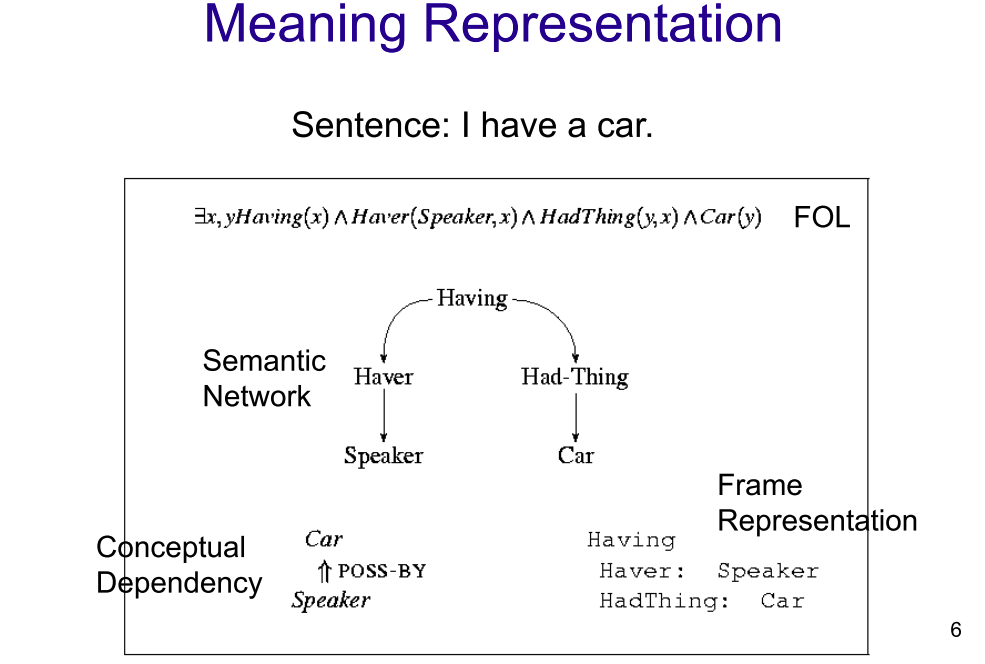
\includegraphics[width=0.8\columnwidth]{meaning-representation}

\subsection{Syntax Driven Semantic Analysis}
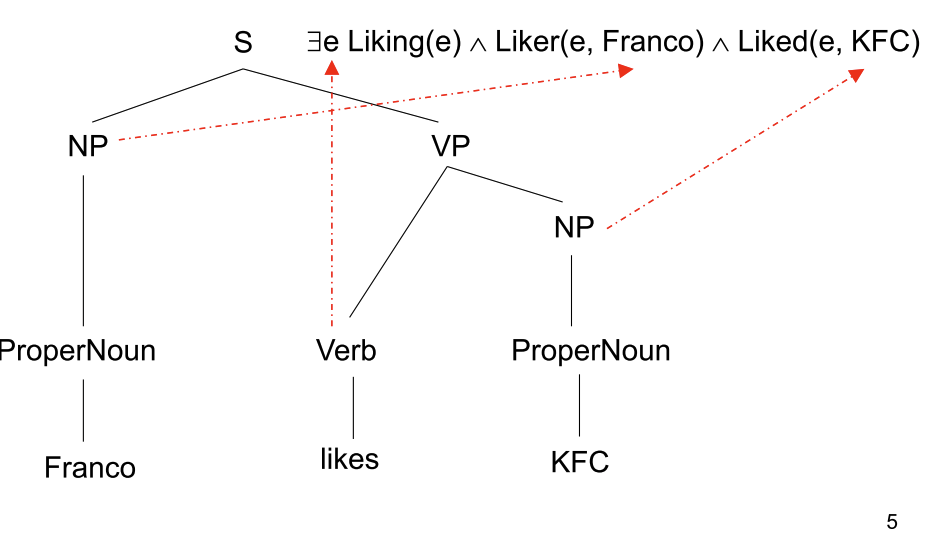
\includegraphics[width=0.8\columnwidth]{syntax-driven-semantic-analysis}


\end{multicols*}
\end{document}
